\section{Локальные поверхностные плазмон-поляритоны}

Поверхностными поляритонами называются волны, распространяющиеся вдоль границы раздела двух различных сред и существующие одновременно в них обеих. Поля, переносимые этими волнами, локализованы вблизи поверхности и затухают по обе стороны от нее \cite{Libenson}. Поверхностными плазмон-поляритонами (ПП) являются поверхностные волны, распространяющиеся вдоль границы раздела сред металл-диэлектрик.

Помимо бегущих вдоль поверхности раздела сред металл-диэлектрик ПП, локализованные поверхностные электромагнитные возбуждения могут существовать и в других объектах, таких как металлические частицы. Такие поверхностные возбуждения в ограниченной геометрии называются локальными поверхностными плазмонами (ЛПП). Частота ЛПП может быть определена в электростатическом приближении из решения уравнения Лапласа с подходящими граничными условиями. Применение электростатического приближения, не учитывающего эффектов запаздывания, возможно при условии, что характерный размер частицы $ a $ много меньше длины волны $ \lambda $ возбуждающего излучения, $ a \ll \lambda $. Для металлических сферических частиц, в которых диэлектрическая проницаемость металла определяется формулой Друде:

\begin{equation}
\varepsilon (\omega) = 1 - \frac{\omega ^2 _p}{\omega ^2} 
\label{eq:EpsilonFreeElectron},
\end{equation}
частота ЛПП находится по формуле:
\begin{equation}
\omega _l = \omega _p \left(\frac{l}{\varepsilon _0 (l + 1) + l}\right)^{1/2},  
\label{eq:FrequencyLocalSPP}
\end{equation}
где $ \omega _p $ --- плазменная частота металла, $  l = 1, 2, 3... $ --- натуральное число, $ \varepsilon _0 $ --- диэлектрическая проницаемость окружающей среды \cite{Zayats}. Для сфер радиуса $ a $ и объема $ V $ Лоренц вывел соотношение для электрической поляризуемости:

\begin{equation}
\alpha = \frac{3 (m^2 - 1)}{4 \pi (m^2 + 2)} V = \frac{m^2 - 1}{m^2 + 2} a^3,
\label{eq:polarizability}
\end{equation}
где $ m = n - ik $ --- комплексный показатель преломления, состоящий из показателя преломления $ n $ и коэффициента экстинкции $ k $.

Для частиц в форме эллипсоида с полуосями $ a $, $ b $ и $ c $ выполняется соотношение, которое дает три главных значения $ \alpha_1 $, $ \alpha_2 $ и $ \alpha_3 $ тензора поляризуемости:
\begin{equation}
\alpha _i = \frac{V}{4 \pi (L_i + \frac{1}{m^2 - 1})},
\label{eq:polarizabilityEllip}
\end{equation}
где $ L_i $ --- фактор деполяризации, зависящий от размеров осей эллипсоида. При произвольном выборе полуосей $ a $, $ b $ и $ c $ получим:
\begin{equation}
L_1 = \int_0^\infty \frac{a b c \mathrm{d} s}{2 (s + a^2)^{3/2} (s + b^2)^{1/2} (s + c^2)^{1/2}},
\label{eq:Lfactor}
\end{equation}
и при циклической перестановке аналогичные формулы для $ L_2 $ и $ L_3 $ \cite{LPP_Hulst}.

\section{Эффекты плазмонной линейки при взаимодействии димера плазмонных наночастиц}

Оптические свойства золотых наночастиц достаточно хорошо изучены и используются во многих областях науки и технологиях, таких как направленная транспортировка лекарственных веществ \cite{drugDelivery}, визуализация клеток \cite{cellImaging}, фототермическая терапия \cite{photothermalTherapy} и других медицинских и биологических направлениях. Современные исследования в области плазмоники сосредоточены в том числе на изучении резонанса ЛПП в ансамблях металлических наночастиц в связи с использованием их, например, в биосенсорике \cite{biosensing}. В этих исследованиях было показано, что электромагнитное взаимодействие между частицами приводит к сдвигу спектрального положения резонанса ЛПП по отношению к положению резонанса ЛПП изолированных наночастиц такой же геометрической формы. На рис.~\ref{img:bioDNA} показано, как между двумя золотыми наночастицами закреплялась молекула ДНК, и ее длина измерялась по смещению положения резонанса ЛПП. Величина сдвига зависит от энергии взаимодействия между наночастицами, которая, в свою очередь, зависит от расстояния между наночастицами. Следовательно, измеряя величину сдвига резонанса, можно определить расстояние между наночастицами. Sonnichsen et al. \cite{bioplasmonruler} и Reinhard et al. \cite{bioplasmonruler2} использовали данное свойство для разработки так называемой  плазмонной линейки для измерения расстояний на наномасштабах, в том числе в биологических системах.
\begin{figure}[h]
\center{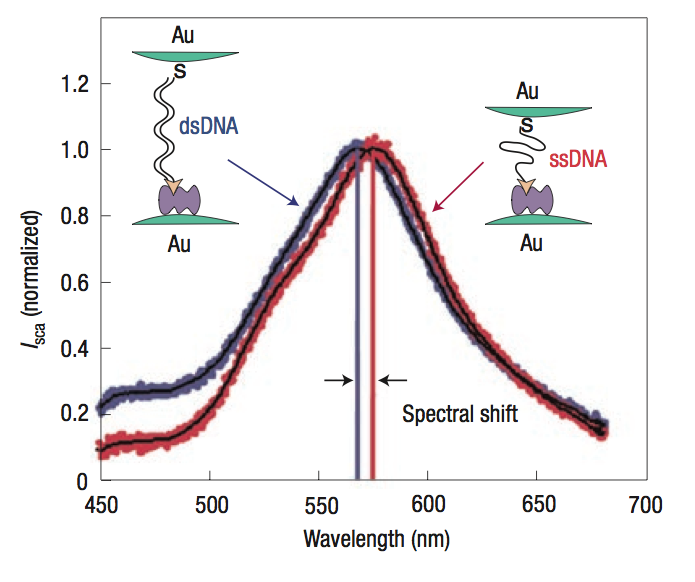
\includegraphics[width=8cm]{img/biosensingDNA.png}}
\caption{Пример спектрального сдвига в системе из двух золотых наночастиц, соединенных между собой одноцепочечной молекулой ДНК (красная линия) и двухцепочечной молекулой ДНК (синяя линия) \cite{biosensing}.}
\label{img:bioDNA}
\end{figure}
Системы из двух оптически связанных наночастиц называются плазмонными димерами. Оптическими свойствами плазмонных димеров можно управлять, изменяя форму наночастиц в димере, их взаиморасположение, поляризацию падающего электромагнитного излучения.

Одними из первых димеров исследовались системы из двух нанодисков. В статье \cite{plasonrulereq} исследуется зависимость положения локального плазмонного резонанса от расстояния между двумя нанодисками из золота. Пары нанодисков из золота располагались на кварцевой подложке и имели толщину 25 нм и диаметр 88 нм. Расстояние между нанодисками варьировалось и составляло 212, 27, 17, 12, 7 и 2 нм. Изображение ансамбля из димеров нанодисков с расстоянием между нанодисками 12 нм, полученное с помощью растрового электронного микроскопа, показано на рис. \ref{img:PR_SEM}.
\begin{figure}
\center{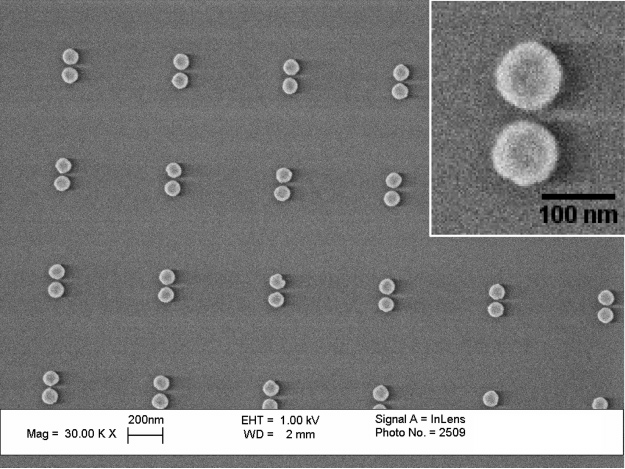
\includegraphics[width=10cm]{img/PR_SEM.png}}
\caption{Изображение пар нанодисков из золота, полученное с помощью растрового электронного микроскопа. Расстояние между нанодисками составляет 12 нм, диаметр нанодиска составляет 88 нм, а толщина --- 25 нм \cite{plasonrulereq}.}
\label{img:PR_SEM}
\end{figure}
Спектры резонансов ЛПП были получены с помощью микроспектроскопии пропускания. При падении света с поляризацией, параллельной оси между центрами нанодисков, наблюдался сдвиг резонанса ЛПП в красную область спектра при уменьшении расстояния между нанодисками. На рис.~\ref{img:PR_extinction} показана зависимость коэффициента экстинкции от длины волны падающего света с поляризацией, параллельной оси между центрами нанодисков, для различных расстояний между нанодисками.
\begin{figure}[t]
\center{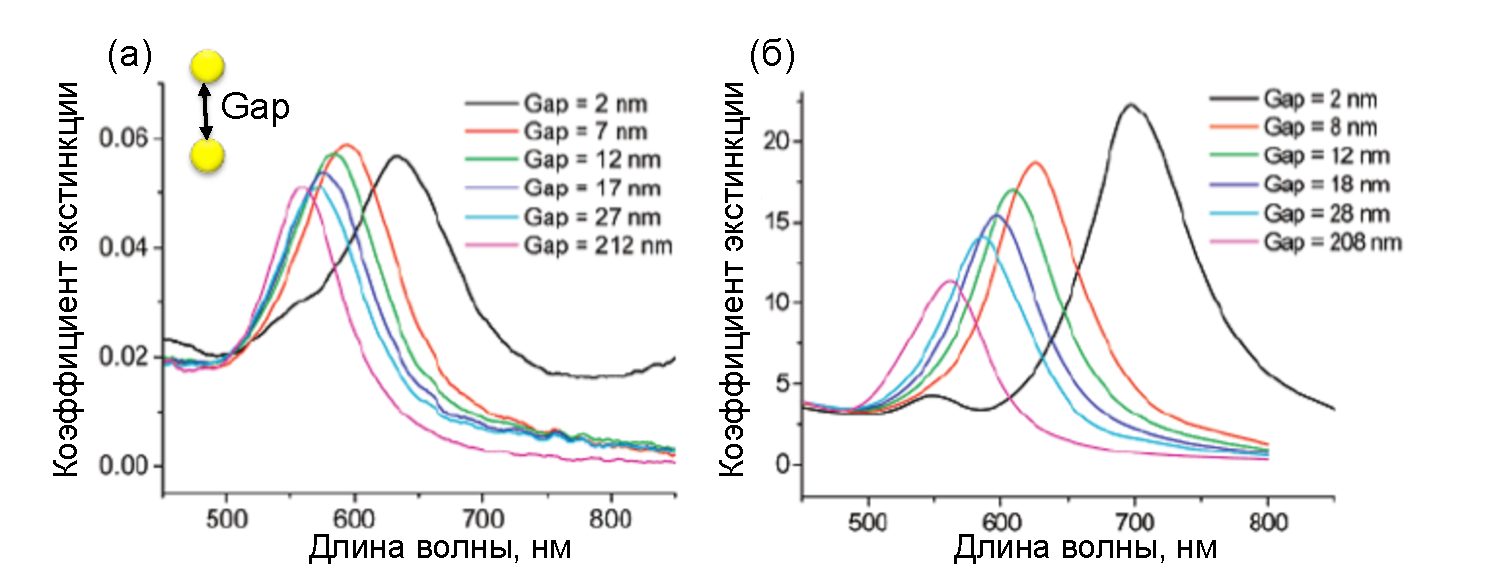
\includegraphics[width=18cm]{img/PR_extinction_ru.pdf}}
\caption{(а) Экспериментальные и (б) численные спектры коэффициента экстинкции при падении света на структуру из димеров нанодисков из золота с различными расстояниями между нанодисками. Поляризация параллельна оси между центрами нанодисков \cite{plasonrulereq}.}
\label{img:PR_extinction}
\end{figure}
\begin{figure}[t]
\center{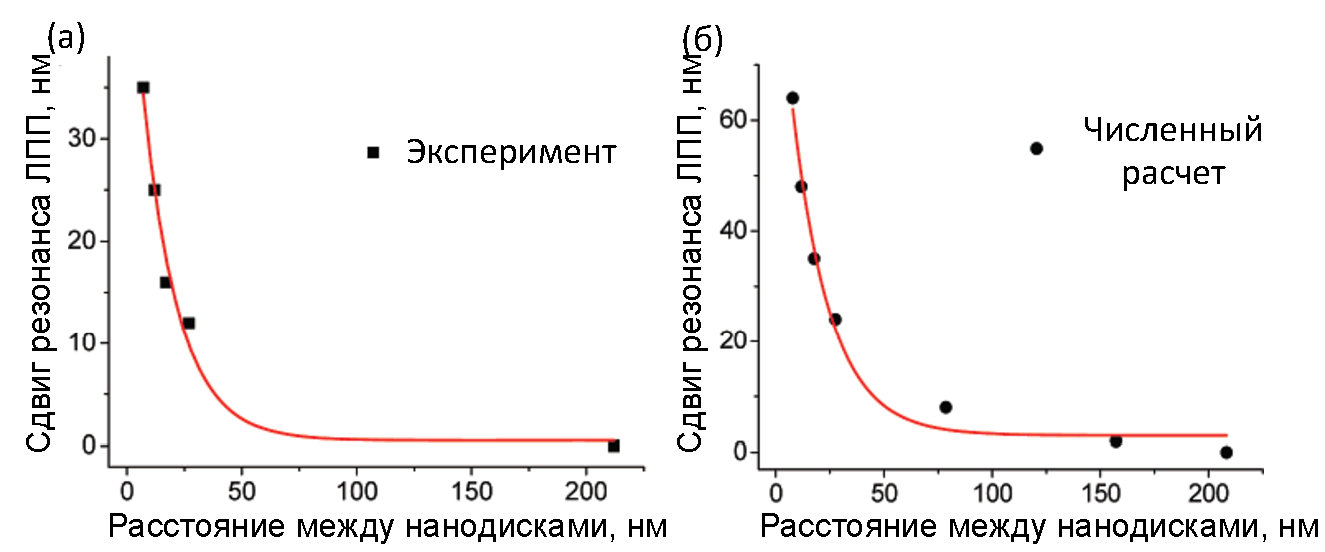
\includegraphics[width=17cm]{img/PR_ruler_ru.pdf}}
\caption{Зависимость сдвига резонанса ЛПП для пар золотых нанодисков от расстояния между нанодисками в эксперименте (а) и численных расчетах (б). Красная линия соответствует кривой $ y = y_0 + a \cdot e^{-x/l} $  \cite{plasonrulereq}.}
\label{img:PR_ruler}
\end{figure}

На рис.~\ref{img:PR_ruler} показана зависимость сдвига резонанса ЛПП от расстояния между нанодисками. Резонанс ЛПП при расстоянии между нанодисками 212 нм был выбран опорным при расчете относительного сдвига, так как взаимодействие между нанодисками можно положить минимальным.

Учитывая данное поведение системы, было выведено следующее феноменологическое уравнение для плазмонной линейки:
\begin{equation}
\frac{\Delta \lambda}{\lambda_0} \approx 0.18 \cdot \exp \left( \frac{-(s/D)}{0.23} \right),
\label{eq:plasmon_ruler}
\end{equation}
где $ \Delta \lambda $ --- величина сдвига резонанса ЛПП, $ \lambda_0 $ --- резонанс ЛПП изолированной наночастицы, $ D $ --- диаметр наночастицы. Такая линейка, например, была использована для измерения длин молекул ДНК \cite{bioplasmonruler3}. Более общее уравнение для плазмонной линейки выглядит следующим образом:
\begin{equation}
\frac{\Delta \lambda}{\lambda_0} = A \cdot \exp \left( \frac{-(s/D)}{\tau} \right),
\label{eq:ruler_general}
\end{equation}
где $ A $ -- предэкспоненциальный множитель, а $ \tau $ -- константа затухания взаимодействия наночастиц в димере.

% Далее описать взаимодействие между димерами наностержней
Димеры из золотых наностержней являются наиболее часто используемыми при исследовании оптических свойств димеров золотых наночастиц. Это связано с тем, что появляется возможность исследовать не только зависимость положения резонанса ЛПП от расстояния между наночастицами, но и изучить поведение резонанса ЛПП при различном взаимном расположении наностержней. Двумя основными видами взаимного расположения пары наностержней являются $ \sigma $-димеры и $ \pi $-димеры. При этом наностержни располагаются наподобие орбитальных $ \sigma $- и $ \pi $- связей, соответственно. В статье \cite{nanorods2} исследуется зависимость положения резонанса ЛПП от расстояния между наностержнями в $ \sigma $-димерах. Массивы из $ \sigma $-димеров располагались на кварцевой подложке и были изготовлены с помощью электронно-лучевой литографии. На рис.~\ref{img:PR_nanorods}(A-C) показаны изображения исследуемых $ \sigma $-димеров, полученные в растровом электронном микроскопе. Поляризация света была линейная вдоль наностержней. Экспериментальные спектры экстинкции $ \sigma $-димеров с различным расстоянием между наностержнями показаны на рис.~\ref{img:PR_nanorods}E. Видно, что при уменьшении расстояния между наностержнями резонанс ЛПП сдвигается в красную область спектра. Экспериментальная и теоретическая зависимости относительного сдвига резонанса ЛПП от нормированного на длину наностержней расстояния между наностержнями показаны на рис.~\ref{img:PR_nanorods}D. Как и в случае димеров нанодисков \cite{plasonrulereq}, наблюдается экспоненциальный спад. Красной сплошной линией на рис.~\ref{img:PR_nanorods}D показано приближение плазмонной линейки, описываемое уравнением (\ref{eq:ruler_general})  с коэффициентом $ \tau = 0.2 $.

\begin{figure}[t]
\center{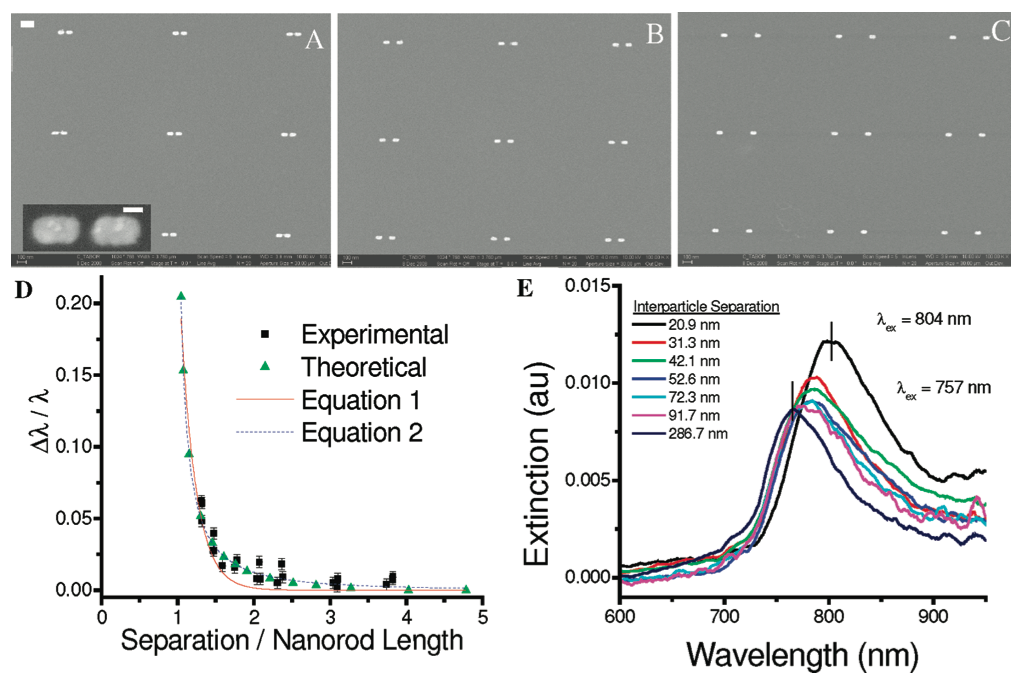
\includegraphics[width=1\linewidth]{img/PR_nanorods.png}}
\caption{(A -- C) Изображения $ \sigma $-димеров, полученные с помощью растрового электронного микроскопа, с расстоянием между наностержнями 20.9, 72.3, 286.7 нм, соответственно. Масштабная линейка в левом верхнем углу рис. A равняется 100 нм. Вставка в рис. A --- увеличенное изображение $ \sigma $-димера в 400000 раз. (D) Зависимость относительного сдвига резонанса ЛПП от нормированного на длину наностержней расстояния между наностержнями. Черными квадратиками нанесены экспериментальные данные, зелеными треугольниками --- расчитанные с помощью метода дискретного дипольного приближения. (E) Экспериментальные спектры экстинкции семи $ \sigma $-димеров с различным расстоянием между наностержнями показывают спектральный сдвиг резонанса ЛПП с 757 нм до 804 нм \cite{nanorods2}.}
\label{img:PR_nanorods}
\end{figure}

Когда две наночастицы, каждая из которых имеет свой резонанс ЛПП, приближаются друг к другу, ближнепольные компоненты поля рассеяния каждой из частиц перекрываются друг с другом, что и влияет на сдвиг резонансов ЛПП. Взаимодействие между двумя вырожденными плазмонными модами можно по аналогии свести к молекулярно-экситонной теории связи \cite{MECT}, которая описывает расщепление энергетического уровня возбужденного состояния на две моды: одну с большей энергией, а вторую с меньшей. При этом ширина полученной энергетической зоны описывается уравнением Симпсона-Петерсона. Аналогично, при взаимодействии двух наночастиц, дипольные моды каждой наночастицы взаимодействуют и преобразуются в две новые дипольные моды димера, одна с большей энергией, другая с меньшей. При этом в случае $ \sigma $-димера мода с большей энергией является антисимметричной и темной, то есть не возбуждающейся плоской волной, а мода с меньшей энергией --- симметричной и светлой.

Также возможны и другие варианты взаимного расположения наностержней. Так, в статье \cite{nanorods1} рассматриваются не только $ \sigma$-димеры, но и $ \pi$-димеры. В случае $ \pi$-димеров симметричная мода имеет большую энергию, чем антисимметричная мода, а значит при уменьшении расстояния между наностержнями резонанс ЛПП должен смещаться в синюю область. На рис.~\ref{img:dimer_resonances} показаны схемы гибридизации димеров наностержней при различном их взаимном расположении. Красным крестом отмечены моды, которые являются темными. При этом небольшой продольный сдвиг стержней в случае $ \pi$-димеров превращает темную моду в светлую, что и показано на рис.~\ref{img:dimer_resonances}b.

\begin{figure}[t]
\center{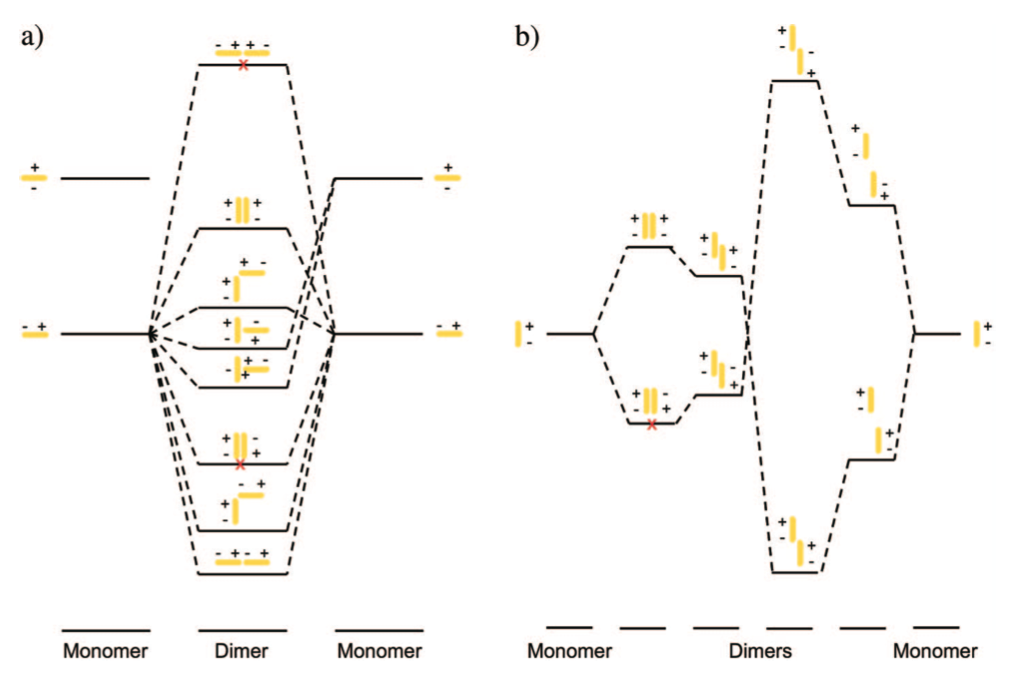
\includegraphics[width=1\linewidth]{img/dimer_resonances.png}}
\caption{Схемы гибридизации димеров наностержней при их различном взаиморасположении. (a) -- $ \sigma$-димеры, (b) -- $ \pi $-димеры \cite{nanorods1}.}
\label{img:dimer_resonances}
\end{figure}

% Новый абзац про резонансы более высоких порядков
%Так, в статье изучаются \cite{nanoring} изучается не только положение резонанса ЛПП в случае дипольной моды, но и в случае более высоких порядков плазмонных мод, а в статье \cite{diffractionCoupling} изучается квадрупольная плазмонная мода. Подробно данная статья описана в обсуждении результатов.
\begin{figure}
\center{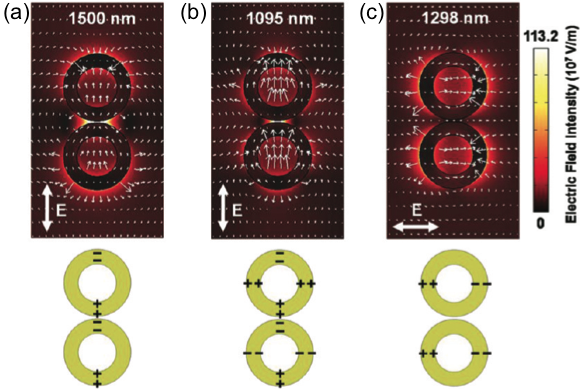
\includegraphics[width=0.6\linewidth]{img/high-order_res.png}}
\caption{Численно рассчитанное распределение интенсивности электромагнитного поля в случае резлнанса ЛПП с дипольной модой (a,c) при падении света с различной линейной поляризацией, и в случае резонанса ЛПП более высокого порядка (b). Ниже представлено мгновенное распределение зарядов для данных плазмонных мод \cite{nanoring}.}
\label{img:high-order_res}
\end{figure}
Помимо резонансов ЛПП с дипольной модой, примеры возбуждения которых в случае $ \sigma $-  и $ \pi $- димеров представлены на рис.~\ref{img:dimer_resonances}, возможно возбуждение резонансов ЛПП более высоких порядков. В статье \cite{nanoring} рассматриваются димеры золотых наноколец, в которых помимо резонанса с дипольной модой (рис.~\ref{img:high-order_res}(a, c)) возбуждался резонанс ЛПП более высокого порядка (рис.~\ref{img:high-order_res}b). При этом резонанс ЛПП более высокого порядка для данного димера также подчинялся уравнению плазмонной линейки (\ref{eq:ruler_general}). В статье \cite{diffractionCoupling} изучается квадрупольная плазмонная мода в нанокольцах.
%Конец нового абзаца

В других работах также исследовалась зависимость сдвига резонанса ЛПП в зависимости от расстояния между наночастицами. При этом частицы были различной геометрической формы, например, нанопризмы \cite{nanoprism, nanoshells}, наносферы \cite{nanospheres, nanospheres2}, наноциллиндры \cite{nanocyllinders} и наностержни \cite{nanorods}. Также исследовался резонанс ЛПП при различных взаимных расположениях двух наночастиц одной геометрической формы \cite{nanorods2, nanorods3, 3druler}. При этом как правило изучалось поведение резонанса в $ \sigma$-димерах, поэтому представляет большой интерес изучение поведения резонанса ЛПП в $ \pi$-димерах, а также взаимодействия наночастиц, в которых возможно возбуждение различных плазмонных мод. 